%% Week 43 -- The Poisson equation three ways (hard and soft constraints
%% against Thomas' algorithm), reading a binary classifier (confusion matrix,
%% ROC, thresholds), and the first hour of convolutional neural networks.
%% Sources: Chapter 9, Sections 9.5 and 9.10 (Poisson equation, physics-
%% informed networks); Chapter 1, Section 1.14 (LU, tridiagonal systems);
%% Chapter 5, Sections 5.12-5.13 (measuring a classifier, the Wisconsin
%% data); Chapter 10, Sections 10.1-10.5 and 10.8 (convolution, the layer,
%% equivariance, pooling, the digits experiment).
%% Part 0 (5 min): the solutions to the exercises of weeks 41 and 42 are out.
%% Part 1 (25 min): the Poisson equation with the trial solution of week 42,
%% with a PINN, and with finite differences solved by Thomas' algorithm.
%% Part 2 (15 min): the confusion matrix, precision/recall/F1, the ROC curve
%% and the AUC, the threshold, the ten-class matrix -- on "is it a five?"
%% with the two classifiers of Project 2.
%% Part 3 (45 min): convolutional neural networks, Chapter 10 up to pooling
%% and the experiment of Section 10.8.
%% Equation, figure, section and table numbers are those of book.aux
%% (2026-09-23; chapters 5, 9 and 10 unchanged since).
%% Figures week43_*.pdf are produced by make_week43_figures.py, which imports
%% the week-41 network and the week-42 differential-equation code; the same
%% code appears verbatim in week43.ipynb.  Book figures come from
%% BookFigures/chapter05_*, chapter09_* and chapter10_*.
%% Tuesday (week43tuesday.tex/ipynb) has ONE case: a binary classifier for
%% Project 2 read through its confusion matrix and ROC curve, which is also
%% the structure of exercisesweek43.ipynb (deadline Friday October 23).
%% Build:  pdflatex week43slides.tex  (twice)
\documentclass[10pt,aspectratio=169]{beamer}
\usetheme{red_plain}
\usepackage[T1]{fontenc}
\usepackage[utf8]{inputenc}
\usepackage{amsmath,amssymb,bm}
\usepackage{graphicx}
\usepackage{listings}
\usepackage{xcolor}
\usepackage{booktabs}
\graphicspath{{../BookFigures/chapter05_logistic_regression/}{../BookFigures/chapter09_differential_equations/}{../BookFigures/chapter10_convolutional_networks/}{./}}

%% ---- code listings
\definecolor{codebg}{rgb}{0.97,0.97,0.97}
\lstset{language=Python,basicstyle=\ttfamily\scriptsize,backgroundcolor=\color{codebg},
  keywordstyle=\color{blue!70!black}\bfseries,commentstyle=\color{green!45!black},
  stringstyle=\color{red!60!black},showstringspaces=false,frame=single,
  framerule=0pt,xleftmargin=4pt,xrightmargin=4pt,breaklines=true,columns=fullflexible}

%% ---- the "pause and think" question frames
\newcounter{insight}
\newenvironment{insight}[1][]{%
  \stepcounter{insight}%
  \begin{frame}{Pause and think \arabic{insight}: #1}%
  \setbeamercolor{block title}{bg=structure.fg,fg=white}%
  \setbeamercolor{block body}{bg=structure.fg!8}%
  \small
}{\end{frame}}
\newcommand{\question}[1]{\begin{block}{Question}#1\end{block}}
\newcommand{\answer}[1]{\pause\begin{block}{Answer}#1\end{block}}
\newcommand{\hint}[1]{\pause{\small\emph{Hint: }#1}}

\setbeamertemplate{footline}[frame number]
\setbeamerfont{block title}{size=\small}
\setbeamertemplate{blocks}[rounded][shadow=false]
\setbeamercovered{invisible}

\title{Week 43: One Equation Three Ways, Reading a Classifier, and Convolutional Networks}
\subtitle{The Poisson equation with hard constraints, soft constraints and
  Thomas' algorithm; what the measures of a classifier mean; and the first
  hour of Chapter 10\\[3pt]
  \small With pauses for questions}
\author{Morten Hjorth-Jensen}
\institute{Department of Physics and Center for Computing in Science Education,\\
  University of Oslo, Norway}
\date{}

\begin{document}

\begin{frame}
\titlepage
\end{frame}

\begin{frame}{Plan for week 43}
\footnotesize
\textbf{Monday lecture (2$\times$45 min):}
\begin{itemize}
  \item \textbf{First, five minutes:} the \emph{solutions} to the exercises
        of weeks 41 and 42 are in the weekly material folders -- where, and
        how to use them
  \item \textbf{One equation three ways (25 min):} the method of week 42
        once more on the one-dimensional Poisson equation -- the trial
        solution that carries the boundary conditions (hard constraints,
        Section 9.5), a physics-informed network that pays for them in the
        cost (soft constraints, Section 9.10), and the classical
        finite-difference solution with its tridiagonal system solved by
        Thomas' algorithm in $\mathcal{O}(n)$ operations (Section 1.14)
  \item \textbf{Reading a classifier (25 min):} a probability is not a
        decision; the four counts of the confusion matrix and what each
        measure made from them \emph{means} -- accuracy and why it misleads,
        precision, recall, specificity, $F_1$, balanced accuracy, MCC -- on a
        worked screening example; the ROC curve and the AUC as a probability
        about pairs, the precision--recall curve, why we train on the cross
        entropy; then all of it at work on ``is this digit a five?'' with
        the two classifiers of Project 2, and the ten-class matrix
        (Section 5.12)
  \item \textbf{Second hour: convolutional neural networks} (Chapter 10,
        Sections 10.1--10.3): why not a dense layer, convolution as
        polynomial multiplication and as a Toeplitz matrix, padding and
        cross-correlation, the layer with channels, output sizes and
        parameter counts, and three filters on a digit -- equivariance and
        pooling follow next week
\end{itemize}
\textbf{Tuesday (flipped classroom):} the worked screening example of today
in full detail, then \emph{one} case: your own confusion matrix, ROC curve
and AUC for a binary classifier of Project 2 -- the structure of this
week's exercises (\textbf{deadline Friday October 23}).\\[2pt]
\textbf{Reading:} Sections 9.5 and 9.10, Section 1.14; Sections 5.12--5.13;
Chapter 10, Sections 10.1--10.3.  Goodfellow et al.\ Chapter 9;
Raschka et al.\ Chapter 14; Hastie et al.\ Section 9.2.5 on the ROC curve.
\end{frame}

\begin{frame}{Before we start: the solutions to weeks 41 and 42 are out}
\small
\begin{columns}[T]
\begin{column}{0.5\textwidth}
\begin{block}{Where}
\footnotesize
In the weekly material folders of the course repository, next to the
exercise notebooks:
\texttt{doc/WeeklyMaterial/week41/}\\
\hspace*{1em}\texttt{exercisesweek41\_solutions.ipynb}\\
\texttt{doc/WeeklyMaterial/week42/}\\
\hspace*{1em}\texttt{exercisesweek42\_solutions.ipynb}\\
in \texttt{github.com/EducationalMaterialUiO/}\\
\hspace*{1em}\texttt{MachineLearningUiO}.
Both are executed notebooks: every number is reproducible with the seed of
the exercise set, and every hand-written gradient is checked against
\texttt{jax.grad}.
\end{block}
\begin{block}{What they contain}
\footnotesize
Week 41: the forward pass for any depth, custom activations, the batched
convention, the iris classifier and why the training accuracy is not a
useful number.  Week 42: the backward pass in six steps, the softmax
shortcut $\bm{\delta}^{L}=\bm{a}^{L}-\bm{y}$, SGD with momentum, the
\texttt{NeuralNetwork} class, and a closing discussion of the eleven
insights the week was meant to give.
\end{block}
\end{column}
\begin{column}{0.48\textwidth}
\begin{block}{How to use them}
\footnotesize
\begin{enumerate}
  \item Not before you have tried.  Compare \emph{your} solution with ours
        afterwards: the shapes, the checks, the numbers.
  \item Where the numbers differ, find out why before reading on -- a
        different seed, a forgotten $2/n$, a transposed weight.
  \item The code is yours to reuse in Project 2 (deadline
        \textbf{November 6}), provided you can explain every line of it.
  \item The closing discussions list what we expect you to be able to say in
        the Tuesday sessions and in the project report.
\end{enumerate}
The week-43 solutions follow after Friday's deadline.
\end{block}
\end{column}
\end{columns}
\end{frame}

%% ====================================================================
%% Part 1: the Poisson equation three ways (25 min)
%% ====================================================================

\begin{frame}{Week 42 in one frame: the equation is the cost (Sections 9.1--9.3)}
\small
\begin{columns}[T]
\begin{column}{0.5\textwidth}
\begin{block}{The recipe}
\scriptsize
Write the equation as a residual $r=0$; write a trial solution
$g_t(x,P)=h_1(x)+h_2(x)N(x,P)$ that satisfies the conditions for every $P$
(Eq.~9.2); evaluate the residual at collocation points $x_i$ and minimise
\[
  C(P)=\frac{1}{N}\sum_i r\bigl(x_i,g_t,g_t',g_t''\bigr)^{2}\qquad(9.3)
\]
with Adam.  No data: the only information is the equation and its
conditions.  The derivatives with respect to the \emph{input} come from
\texttt{jax.grad} nested (\texttt{d\_dxk}), or from the forward recursions
(9.5)--(9.6); the hidden activation must have an $f''$, so $\tanh$.
\end{block}
\begin{block}{Last week's result for Poisson}
\scriptsize
$-g''=(3x+x^{2})e^{x}$ on $(0,1)$ with $g(0)=g(1)=0$, exact
$g=x(1-x)e^{x}$ (9.15)--(9.17); $g_t=x(1-x)N$ (9.18); $[1,30,30,1]$, sixty
points, $4000$ iterations: max error $1.2\times10^{-5}$, against
$2.2\times10^{-5}$ for finite differences with a hundred intervals.
\end{block}
\end{column}
\begin{column}{0.48\textwidth}
\begin{block}{Today's question}
\scriptsize
Last week the finite-difference line in the table was a black box: ``a
tridiagonal system, solved in $\mathcal{O}(n)$''.  Today we open the box,
solve the same equation a third way -- with the conditions as \emph{soft}
constraints, as in the physics-informed networks of Section 9.10 -- and put
the three side by side on cost, accuracy and what each one needs from us:
\begin{center}
\begin{tabular}{@{}lll@{}}
\toprule
 & conditions & unknowns\\
\midrule
hard & in $g_t$, exact & $P$ (the network)\\
soft & in the cost, $\lambda$ & $P$ (the network)\\
Thomas & in the matrix, exact & $u_1,\dots,u_{n-1}$\\
\bottomrule
\end{tabular}
\end{center}
\end{block}
\begin{block}{Why it matters for the rest of the course}
\scriptsize
The same three choices -- build structure into the model, pay for it in the
cost, or use a method that has it already -- return in every chapter.  The
convolutional layer of the second hour is the first choice made for
images.
\end{block}
\end{column}
\end{columns}
\end{frame}

\begin{frame}[fragile]{The classical way: finite differences and a tridiagonal system (9.20)--(9.22)}
\begin{columns}[T]
\begin{column}{0.47\textwidth}
\scriptsize
Taylor-expand $u(x_i\pm\Delta x)$ and add; the odd terms cancel,
\[
  u_i''=\frac{u_{i+1}-2u_i+u_{i-1}}{\Delta x^{2}}+\mathcal{O}(\Delta x^{2}),
  \qquad(9.21)
\]
and with $u_0=u_n=0$ the equation $-u''=f$ becomes the tridiagonal system
(9.22), $\tfrac{1}{\Delta x^{2}}(-u_{i-1}+2u_i-u_{i+1})=f_i$ for
$i=1,\dots,n-1$: sub-diagonal $a_i=-1/\Delta x^{2}$, diagonal
$b_i=2/\Delta x^{2}$, super-diagonal $c_i=-1/\Delta x^{2}$.
\begin{block}{Thomas' algorithm: computed, not searched for}
\scriptsize
Gaussian elimination (Section 1.14) on three diagonals never creates a
non-zero outside them.  One forward sweep removes the sub-diagonal,
\[
  c_i'=\frac{c_i}{b_i-a_ic_{i-1}'},\qquad
  d_i'=\frac{d_i-a_id_{i-1}'}{b_i-a_ic_{i-1}'},
\]
and back substitution $u_i=d_i'-c_i'u_{i+1}$ finishes: about $8n$ flops
and $3n$ numbers stored, against $\tfrac{2}{3}n^{3}$ and $n^{2}$ for the
full matrix.  No pivoting: the matrix is symmetric positive definite and
diagonally dominant, so the pivots never get small.
\end{block}
\end{column}
\begin{column}{0.51\textwidth}
\begin{lstlisting}
def thomas(a, b, c, d):
    n = len(d); cp, dp = np.empty(n), np.empty(n)
    cp[0], dp[0] = c[0] / b[0], d[0] / b[0]
    for i in range(1, n):            # forward sweep
        m = b[i] - a[i] * cp[i - 1]
        cp[i] = c[i] / m if i < n - 1 else 0.0
        dp[i] = (d[i] - a[i] * dp[i - 1]) / m
    u = np.empty(n); u[-1] = dp[-1]
    for i in range(n - 2, -1, -1):   # back substitution
        u[i] = dp[i] - cp[i] * u[i + 1]
    return u

def fd_poisson_thomas(n):
    dx = 1.0 / n
    x = np.linspace(0, 1, n + 1); xi = x[1:-1]
    a = c = -np.ones(n - 1) / dx**2
    b = 2 * np.ones(n - 1) / dx**2
    u = np.zeros(n + 1)
    f = (3 * xi + xi**2) * np.exp(xi)
    u[1:-1] = thomas(a, b, c, f)
    return x, u
\end{lstlisting}
\end{column}
\end{columns}
\end{frame}

\begin{frame}{Thomas against the dense solve: accuracy and time (\texttt{fd\_table})}
\small
\begin{columns}[T]
\begin{column}{0.5\textwidth}
\begin{center}
\scriptsize
\setlength{\tabcolsep}{4pt}
\begin{tabular}{@{}rrrr@{}}
\toprule
intervals $n$ & max error & Thomas & dense LU\\
\midrule
$10$ & $2.15\times10^{-3}$ & $0.05$ ms & $0.07$ ms\\
$20$ & $5.41\times10^{-4}$ & $0.04$ ms & $0.05$ ms\\
$50$ & $8.66\times10^{-5}$ & $0.08$ ms & $0.06$ ms\\
$100$ & $2.17\times10^{-5}$ & $0.16$ ms & $0.25$ ms\\
$1000$ & $2.17\times10^{-7}$ & $1.1$ ms & $34$ ms\\
$10\,000$ & $2.16\times10^{-9}$ & $11$ ms & $800$ MB\\
\midrule
hard network, 4000 it. & $1.18\times10^{-5}$ & \multicolumn{2}{c}{$2.7$ s}\\
soft $\lambda=10$, 4000 it. & $4.84\times10^{-5}$ & \multicolumn{2}{c}{$2.4$ s}\\
\bottomrule
\end{tabular}
\end{center}
\scriptsize
Wall-clock times in the lecture container, averaged over five runs; the
dense solve is \texttt{np.linalg.solve} on the full matrix, the network
times are whole Adam runs with \texttt{jax.jit} ($[1,30,30,1]$, sixty
points).
\end{column}
\begin{column}{0.48\textwidth}
\begin{block}{Reading the table}
\scriptsize
The error falls by four when $\Delta x$ halves and by a hundred when $n$
grows tenfold: $\mathcal{O}(\Delta x^{2})$, as (9.21) promised.  Thomas'
time grows linearly -- ten times the points, ten times the time -- while
the dense solve grows as $n^{3}$ and runs out of memory before it runs out
of patience: $n^{2}$ doubles at $n=10^{4}$ is $800$ MB for a matrix with
$3n$ non-zeros.
\end{block}
\begin{block}{Where the network stands}
\scriptsize
With sixty points and four thousand iterations it reaches the accuracy of
$n\approx100$, in $2.7$ s against $0.16$ ms: four orders of magnitude
slower for the same error, and nowhere near $n=10\,000$.  On this problem
the classical method wins by every measure, and we say so: the network is
not for problems that have a Thomas' algorithm.  Section 9.9 lists the
problems that do not -- high dimensions, irregular domains, inverse
problems with data -- and the soft constraints of the next frame are the
entry ticket to them.
\end{block}
\end{column}
\end{columns}
\end{frame}

\begin{frame}[fragile]{The third way: the boundary conditions as soft constraints (Section 9.10)}
\begin{columns}[T]
\begin{column}{0.47\textwidth}
\scriptsize
Drop the scaffolding $x(1-x)$ and let the network be the solution,
$u(x)=N(x,P)$ (Eq.~9.34).  Nothing now enforces $u(0)=u(1)=0$, so we
\emph{ask} the optimiser for it, one least-squares term per condition
(Eqs.~9.35, 9.37, 9.38):
\begin{align*}
  L_{\mathrm{PDE}}&=\frac{1}{N_{\mathrm{col}}}\sum_{i}\bigl(-N''(x_i)-f(x_i)\bigr)^{2},\\
  L_{\mathrm{BC}}&=\tfrac{1}{2}\bigl[N(0)^{2}+N(1)^{2}\bigr],\qquad
  \boxed{\;L=L_{\mathrm{PDE}}+\lambda\,L_{\mathrm{BC}}\;}
\end{align*}
Two point sets instead of one: $58$ interior collocation points and the
two end points.  The weight $\lambda$ plays the part of the Ridge penalty:
how much a boundary error costs relative to an equation error.  The code
of week 42 (\texttt{pinn\_solve}) takes a list of (weight, residual,
points) terms; nothing else changes.
\begin{block}{Hard versus soft, in one sentence each}
\scriptsize
Hard: the conditions hold exactly for every $P$, and the optimiser only
has to solve the equation.  Soft: the conditions hold approximately at the
optimum, the optimiser has to trade them against the equation, and we have
to choose the exchange rate $\lambda$.
\end{block}
\end{column}
\begin{column}{0.51\textwidth}
\begin{lstlisting}
def u_1d(layers, X):       # Eq. (9.34): the network IS u
    return network(layers, X, "tanh")

def r_poisson_pinn(layers, X):   # -u'' - f, nested jax.grad
    d2u = d_dxk(d_dxk(u_1d, 0), 0)(layers, X)
    return -d2u - poisson_f(X[:, 0])

def solve_poisson_soft(lam=10.0, n_iter=4000, seed=1):
    x = np.linspace(0, 1, 60)[:, None]
    X_col = jnp.asarray(x[1:-1])        # 58 interior points
    X_bc = jnp.asarray(x[[0, -1]])      # the two ends
    terms = [("pde", 1.0, r_poisson_pinn, X_col),
             ("bc", lam, u_1d, X_bc)]
    rng = np.random.default_rng(seed)
    layers, hist = pinn_solve(terms, [1, 30, 30, 1],
                              "tanh", n_iter=n_iter,
                              gamma=1e-2, rng=rng)
    ...
\end{lstlisting}
\scriptsize
Last week \texttt{trial\_poisson} returned \texttt{x * (1 - x) * network(...)};
the residual of the \emph{equation} is the same function in both, only who
is responsible for the boundary changed.
\end{column}
\end{columns}
\end{frame}

\begin{frame}{Three solutions of one equation (\texttt{week43\_poisson.pdf})}
\begin{center}
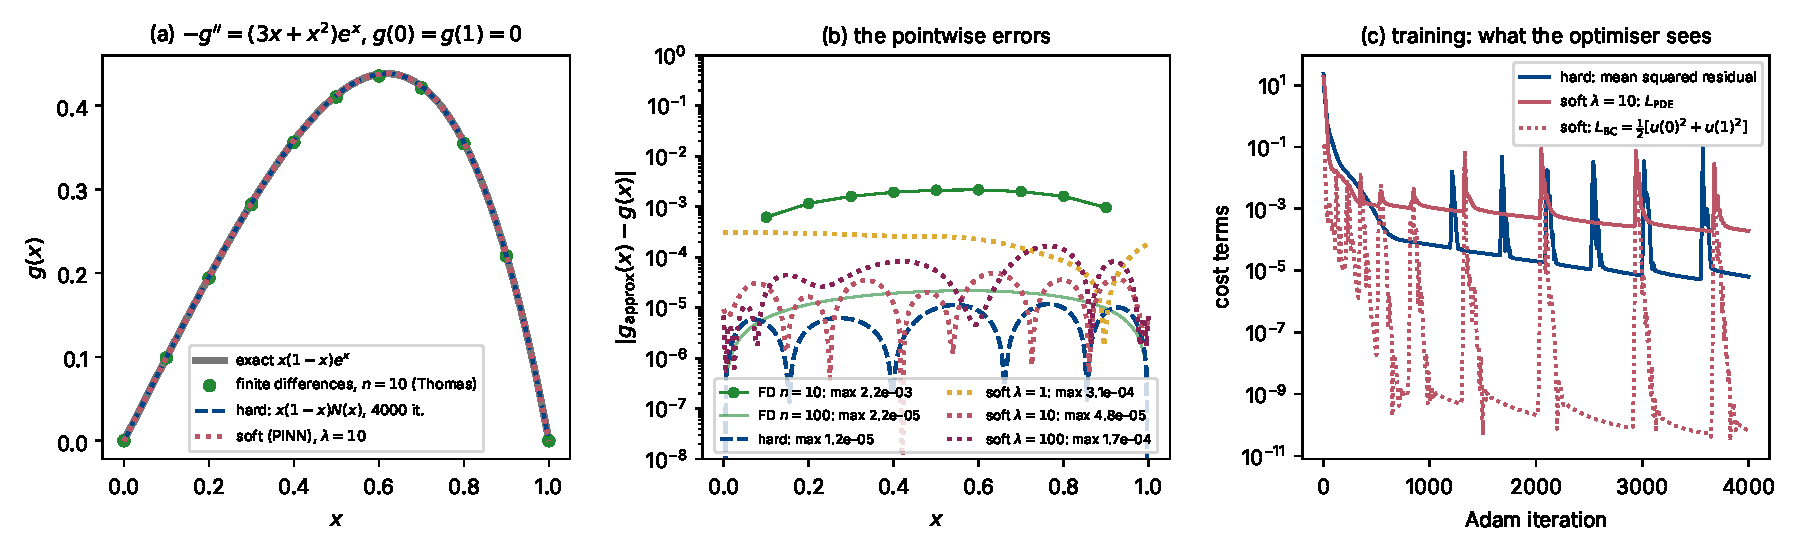
\includegraphics[width=0.99\textwidth]{week43_poisson}
\end{center}
\scriptsize
(a) All four curves lie on the exact solution to the width of the line.
(b) The errors tell them apart: finite differences with $n=10$ at
$2\times10^{-3}$ and $n=100$ at $2\times10^{-5}$, the hard network at
$1.2\times10^{-5}$, the soft one at $4.8\times10^{-5}$ for $\lambda=10$ --
and the soft error for $\lambda=1$ is \emph{largest at the ends},
$3\times10^{-4}$ at $x=0$, exactly where the hard solution is zero by
construction.  (c) What the two optimisers see: the hard cost is one
number; the soft cost is two, and $L_{\mathrm{BC}}$ is driven to
$10^{-11}$ while $L_{\mathrm{PDE}}$ stalls thirty times above the hard
residual.  The spikes are Adam at $\gamma=0.01$ overshooting in a narrow
valley, as in week 38.
\end{frame}

\begin{frame}{Reading the numbers: what $\lambda$ buys and what it costs}
\small
\begin{columns}[T]
\begin{column}{0.5\textwidth}
\begin{center}
\scriptsize
\setlength{\tabcolsep}{3pt}
\begin{tabular}{@{}lcccc@{}}
\toprule
 & max err & $|u(0)|$ & $|u(1)|$ & $L_{\mathrm{PDE}}$\\
\midrule
hard & $1.2\cdot10^{-5}$ & $0$ & $0$ & $6.4\cdot10^{-6}$\\
soft, $\lambda=1$ & $3.1\cdot10^{-4}$ & $3.1\cdot10^{-4}$ & $1.8\cdot10^{-4}$ & $2.2\cdot10^{-5}$\\
soft, $\lambda=10$ & $4.8\cdot10^{-5}$ & $9\cdot10^{-6}$ & $7\cdot10^{-6}$ & $1.9\cdot10^{-4}$\\
soft, $\lambda=100$ & $1.7\cdot10^{-4}$ & $7\cdot10^{-6}$ & $9\cdot10^{-6}$ & $8.6\cdot10^{-4}$\\
\bottomrule
\end{tabular}
\end{center}
\scriptsize
Same network, same $\tanh$, same Adam, same seed, $4000$ iterations each;
$L_{\mathrm{PDE}}$ is the final unweighted equation term, and
$L_{\mathrm{BC}}$ ends at $7\cdot10^{-8}$ for $\lambda=1$ and below
$10^{-10}$ for $\lambda\ge10$.
\end{column}
\begin{column}{0.48\textwidth}
\begin{block}{Three observations}
\scriptsize
\begin{enumerate}
  \item \textbf{Small $\lambda$: the boundary is the error.}  With
        $\lambda=1$ the equation is satisfied better than with any other
        $\lambda$ ($L_{\mathrm{PDE}}=2\times10^{-5}$) and the solution is
        the worst, because it is off by $3\times10^{-4}$ at $x=0$: a
        second-order equation with inexact boundary values has an inexact
        solution everywhere.
  \item \textbf{Large $\lambda$: the equation is the error.}  With
        $\lambda=100$ the boundary values are as good as with $10$ but
        $L_{\mathrm{PDE}}$ is forty times the hard residual -- the gradient
        of $\lambda L_{\mathrm{BC}}$ dominates and one $\gamma$ cannot serve
        both terms (conditioning, Section 4.5; Table 9.1 last week).
  \item \textbf{The best soft solution is four times worse than the hard
        one} and we had to try three values of $\lambda$ to find it.  Where
        a trial solution exists, it is free and exact; where it does not --
        curved boundaries, inverse problems -- the soft version is the one
        we have.
\end{enumerate}
\end{block}
\end{column}
\end{columns}
\end{frame}


%% ====================================================================
%% Part 2: reading a classifier (15 min)
%% ====================================================================

\begin{frame}{A probability is not a decision (Section 5.12)}
\small
\begin{columns}[T]
\begin{column}{0.5\textwidth}
\begin{block}{What the sigmoid head of week 41 gives us}
\scriptsize
For a binary problem the network outputs $p=\sigma(z^{L})\in(0,1)$, trained
with the cross entropy.  To \emph{classify} we must choose a threshold $t$
and declare $\tilde{y}=1$ if $p>t$.  Nothing in the training picked $t$;
$0.5$ is a convention, not a result.
\end{block}
\begin{block}{What this part is about}
\scriptsize
Once a decision is made, every sample lands in one of four boxes -- the
confusion matrix -- and every number people quote (accuracy, precision,
recall, specificity, $F_1$, balanced accuracy, MCC) is a function of those
four counts.  We go through what each one \emph{means} on a worked
example, then through the two curves that judge the scores \emph{before}
any decision is made (ROC and precision--recall), then back to MNIST to
see all of it at work, and finally to the ten-class matrix Project 2 asks
for.
\end{block}
\end{column}
\begin{column}{0.48\textwidth}
\begin{block}{The example of today: is this digit a five?}
\scriptsize
Full MNIST, $y=1$ for the $5421$ fives among $60\,000$ training images
($9.0\%$) and the $892$ among $10\,000$ test images ($8.9\%$).  Two
classifiers from Project 2, the week-41 code unchanged, ten epochs of SGD
with $M=100$, $\gamma=0.1$, seed $2026$:
\begin{center}
\setlength{\tabcolsep}{4pt}
\begin{tabular}{@{}lrr@{}}
\toprule
 & parameters & test acc.\\
\midrule
logistic regression, $784\to1$ & $785$ & $0.9739$\\
one hidden layer, $784\to32\to1$ & $25\,153$ & $0.9932$\\
\midrule
\emph{never say five} & $0$ & $0.9108$\\
\bottomrule
\end{tabular}
\end{center}
The last line is the number every accuracy on this problem must be compared
with: it is what one gets for free.  The imbalance is deliberate -- it is
the situation in which accuracy misleads, and the one you will meet in
every one-against-the-rest reading of a ten-class matrix.
\end{block}
\end{column}
\end{columns}
\end{frame}

\begin{frame}{The confusion matrix: four counts, and what each one means (Eq.~5.67)}
\small
\begin{columns}[T]
\begin{column}{0.46\textwidth}
\begin{block}{Everything starts here}
\scriptsize
\[
  \begin{array}{c|cc}
     & \text{predicted } 1 & \text{predicted } 0\\
    \hline
    \text{true } 1 & \mathrm{TP} & \mathrm{FN}\\
    \text{true } 0 & \mathrm{FP} & \mathrm{TN}
  \end{array}
\]
Rows are the truth, columns the decision.  The diagonal is what went
right; the two off-diagonal entries are the two \emph{kinds} of error, and
they are rarely equally costly.  Every number of this part is a function of
these four counts, and reporting the matrix itself is almost always more
informative than any one of them.  (Mind the layout:
\texttt{sklearn.metrics.confusion\_matrix} puts class $0$ first, rows true
$0/1$, columns predicted $0/1$, so TP is in the lower right.)
\end{block}
\end{column}
\begin{column}{0.52\textwidth}
\begin{block}{In words, for a screening test}
\scriptsize
\begin{itemize}
  \item \textbf{TP}, true positive: has the condition, test says so.  Found.
  \item \textbf{FN}, false negative: has the condition, test says healthy.
        \emph{Missed} -- the dangerous error in screening.
  \item \textbf{FP}, false positive: healthy, test says condition.  A
        \emph{false alarm} -- costs a follow-up, not a life.
  \item \textbf{TN}, true negative: healthy, test says healthy.  Correctly
        left alone.
\end{itemize}
\end{block}
\begin{block}{A worked example we carry through the next frames}
\scriptsize
A test for a condition with prevalence $\pi=2\%$, applied to $1000$
people:
\[
  \mathrm{TP}=15,\quad \mathrm{FN}=5,\quad \mathrm{FP}=40,\quad \mathrm{TN}=940 .
\]
Twenty people have the condition; the test finds fifteen of them and
raises forty false alarms.  Next to it we keep the ``test'' that declares
everybody healthy: $\mathrm{TP}=0$, $\mathrm{FN}=20$, $\mathrm{FP}=0$,
$\mathrm{TN}=980$.
\end{block}
\end{column}
\end{columns}
\end{frame}

\begin{frame}{Accuracy: the number everybody reports, and what it hides (Eq.~5.68)}
\small
\begin{columns}[T]
\begin{column}{0.5\textwidth}
\begin{block}{Definition and meaning}
\scriptsize
\[
  \mathrm{accuracy}=\frac{\mathrm{TP}+\mathrm{TN}}{\mathrm{TP}+\mathrm{TN}+\mathrm{FP}+\mathrm{FN}}
  =\frac{1}{n}\sum_{i=1}^{n}I(y_i=\tilde y_i):
\]
the fraction of decisions that were right, all samples counted alike.  It
is the right number when the classes are balanced \emph{and} the two
errors cost the same.  Otherwise it answers a question nobody asked.
\end{block}
\begin{block}{The worked example}
\scriptsize
Our test: $(15+940)/1000=\mathbf{0.955}$.  The test that declares
everybody healthy: $980/1000=\mathbf{0.980}$ -- \emph{higher}, while
finding nobody.  Accuracy prefers the useless test.
\end{block}
\begin{block}{Always compare with the majority class}
\scriptsize
The majority rule scores $\max(\pi,1-\pi)$ for free; an accuracy means
something only as the fraction of the \emph{remaining} error removed,
$1-(1-\mathrm{acc})/(1-p_0)$.  Our test removed none of it (it added some).
\end{block}
\end{column}
\begin{column}{0.48\textwidth}
\begin{block}{Why: accuracy is a prevalence-weighted average}
\scriptsize
Write $n_+=\mathrm{TP}+\mathrm{FN}$ and $n_-=\mathrm{FP}+\mathrm{TN}$, so
$\pi=n_+/n$.  Then
\begin{align*}
  \mathrm{accuracy}&=\frac{\mathrm{TP}}{n}+\frac{\mathrm{TN}}{n}
   =\frac{n_+}{n}\frac{\mathrm{TP}}{n_+}+\frac{n_-}{n}\frac{\mathrm{TN}}{n_-}\\
  &=\boxed{\;\pi\,\mathrm{recall}+(1-\pi)\,\mathrm{specificity}\;}
\end{align*}
With $\pi=0.02$: $0.02\times0.75+0.98\times0.959=0.955$.  The recall --
how many of the sick we found -- enters with weight $0.02$; whatever the
test does on the sick is invisible at the second decimal.  That is the
whole problem with accuracy under imbalance, in one line.
\end{block}
\begin{block}{Balanced accuracy: the same average with equal weights}
\scriptsize
$\tfrac12(\mathrm{recall}+\mathrm{specificity})$: the accuracy the test
\emph{would} have had on a balanced population.  Our test: $0.855$; the
everybody-healthy test: $\tfrac12(0+1)=0.5$, the score of a coin.  The
first number that tells the two apart.
\end{block}
\end{column}
\end{columns}
\end{frame}

\begin{frame}{Precision and recall: two questions with two denominators (Eq.~5.69)}
\small
\begin{columns}[T]
\begin{column}{0.5\textwidth}
\begin{block}{Recall (sensitivity, true positive rate)}
\scriptsize
$\mathrm{recall}=\mathrm{TP}/(\mathrm{TP}+\mathrm{FN})=\mathrm{TP}/n_+$.
\emph{Of those who have the condition, what fraction did we find?}  The
denominator is the truth; the number is about the \emph{misses}.  Worked
example: $15/20=0.75$ -- one patient in four goes home undetected.  Its
mirror image for the negatives is the specificity,
$\mathrm{TN}/(\mathrm{TN}+\mathrm{FP})=940/980=0.959$: of the healthy, how
many were left alone?  Its complement $\mathrm{FPR}=0.041$ is the
horizontal axis of the ROC curve.
\end{block}
\begin{block}{Precision (positive predictive value)}
\scriptsize
$\mathrm{precision}=\mathrm{TP}/(\mathrm{TP}+\mathrm{FP})$.
\emph{Of those we flagged, what fraction really had it?}  The denominator
is our decision; the number is about the \emph{false alarms}.  Worked
example: $15/55=0.27$ -- three of four people called back are healthy.
This is what a patient with a positive result wants to know, and it is
small because the condition is rare: $40$ false alarms from $980$ healthy
people is only a $4\%$ false positive rate.
\end{block}
\end{column}
\begin{column}{0.48\textwidth}
\begin{block}{They trade against each other}
\scriptsize
Lower the threshold: more samples flagged, more of the sick found (recall
up), more healthy called back (precision down).  Raise it: the reverse.
Which matters is a question about the \emph{application}, not the model:
screening for a serious disease wants recall (a miss is the costly
error); a spam filter wants precision (a lost genuine mail is).
\end{block}
\begin{block}{$F_1$: one number from the two, Eq.~(5.70)}
\scriptsize
\[
  F_1=\frac{2\,\mathrm{prec}\cdot\mathrm{rec}}{\mathrm{prec}+\mathrm{rec}}
  =\frac{2m}{1+m/M},\quad m=\min,\ M=\max,
\]
so $m\le F_1\le 2m$: $F_1$ is \emph{small whenever either is small}.
That is why the harmonic mean: with precision $1$ and recall $0.1$ the
arithmetic mean says $0.55$, the harmonic mean $0.18$ -- perfect on one
axis and useless on the other is useless.  Worked example:
$2\times0.273\times0.75/1.023=0.40$; everybody-healthy: $0$.  $F_1$ never
looks at TN: usable under imbalance, blind to the negatives.
\end{block}
\end{column}
\end{columns}
\end{frame}

\begin{frame}{The worked example in one table, and the correlation coefficient}
\small
\begin{columns}[T]
\begin{column}{0.5\textwidth}
\begin{center}
\scriptsize
\setlength{\tabcolsep}{5pt}
\begin{tabular}{@{}lcc@{}}
\toprule
measure & our test & everybody healthy\\
\midrule
accuracy & $0.955$ & $\mathbf{0.980}$\\
precision & $0.273$ & $0$ ($0/0$)\\
recall & $0.750$ & $0$\\
specificity & $0.959$ & $1.000$\\
$F_1$ & $0.400$ & $0$\\
balanced accuracy & $0.855$ & $0.500$\\
MCC & $0.436$ & $0$\\
\bottomrule
\end{tabular}
\end{center}
\scriptsize
$\mathrm{TP}=15$, $\mathrm{FN}=5$, $\mathrm{FP}=40$, $\mathrm{TN}=940$,
prevalence $2\%$; the empty rule's precision is $0/0$, by convention $0$.
What each row asks: decisions right, all alike; flagged -- how many were?;
sick -- how many found?; healthy -- how many left alone?; both of the
previous two; accuracy at equal class weights; correlation of $y$ and
$\tilde y$.
\end{column}
\begin{column}{0.48\textwidth}
\begin{block}{The Matthews correlation coefficient}
\scriptsize
\begin{gather*}
  \mathrm{MCC}=\frac{\mathrm{TP}\cdot\mathrm{TN}-\mathrm{FP}\cdot\mathrm{FN}}{\sqrt{D}},\\
  D=(\mathrm{TP}+\mathrm{FP})(\mathrm{TP}+\mathrm{FN})(\mathrm{TN}+\mathrm{FP})(\mathrm{TN}+\mathrm{FN}),
\end{gather*}
is exactly the Pearson correlation between the $0/1$ labels $y_i$ and the
$0/1$ decisions $\tilde y_i$ (Section 2.4): $+1$ perfect, $0$ no
relation, $-1$ perfectly wrong.  It uses all four counts and is symmetric
in the two classes, so it is the one scalar that is hard to fool by
imbalance: $(15\cdot940-40\cdot5)/\sqrt{55\cdot20\cdot980\cdot945}=0.436$,
against $0$ for the empty rule (its numerator is $0\cdot980-0\cdot20$).
\end{block}
\begin{block}{Reading the table}
\scriptsize
Accuracy ranks the two tests the wrong way round; every other row ranks
them the right way, and each says something different: three quarters of
the sick found (recall), three false alarms per true case (precision), a
weak but real association between test and truth (MCC).  Which to
\emph{report} depends on who is asking; the matrix contains all of them.
\end{block}
\end{column}
\end{columns}
\end{frame}

\begin{frame}{The ROC curve and the AUC: what they measure}
\small
\begin{columns}[T]
\begin{column}{0.5\textwidth}
\begin{block}{The curve}
\scriptsize
Every threshold $t$ gives one confusion matrix, hence one point
$(\mathrm{FPR},\mathrm{TPR})$; sweeping $t$ from $1$ to $0$ traces the
\emph{receiver operating characteristic} from $(0,0)$ (flag nobody) to
$(1,1)$ (flag everybody).  A perfect ranking passes through $(0,1)$, a
random one gives the diagonal.  The curve is every trade-off between
misses and false alarms the model offers; a threshold picks one point.
\end{block}
\begin{block}{The area: a probability about pairs}
\scriptsize
$\mathrm{AUC}=\mathrm{Prob}(\text{a random positive outscores a random
negative})$.  Sort all $n=n_++n_-$ scores increasingly; let $R_i$ be the
rank of the $k_i$th positive.  Below it sit $R_i-1$ samples, $k_i-1$ of
them positives, so it outranks $R_i-k_i$ negatives.  Summed over the
positives: $\sum_iR_i-\tfrac12n_+(n_++1)$ correctly ordered pairs of
$n_+n_-$, hence
\[
  \mathrm{AUC}=\frac{\sum_{i\in\mathrm{pos}}R_i-\tfrac12n_+(n_++1)}{n_+n_-},
\]
the Mann--Whitney statistic (ties: average rank, half a pair) -- equal to
the trapezoidal area under the curve.
\end{block}
\end{column}
\begin{column}{0.48\textwidth}
\begin{block}{What the AUC does and does not depend on}
\scriptsize
Only on the \emph{ranking} of the scores.  Not on $t$ -- there is no
threshold in it.  Not on the prevalence: duplicate every positive and TP
and FN double together, so $\mathrm{TPR}$ is unchanged at every $t$, and
$\mathrm{FPR}$ never saw the positives.  A random ranking gives $0.5$; so
does a classifier whose scores are all equal (every $R_i=(n+1)/2$);
$1$ is perfect, and $0$ means the scores are perfectly wrong -- flip them.
\end{block}
\begin{block}{The precision--recall curve is different}
\scriptsize
Same sweep, precision on the vertical axis.  Precision has FP in its
denominator, so the ratio of positives to negatives enters it: duplicate
the positives and the curve moves up.  Its floor is the prevalence (flag
everybody: precision $=\pi$), so it is the curve to look at when positives
are rare and the ROC curve flatters -- a $1\%$ false positive rate on
$9108$ negatives is $91$ false alarms against $892$ fives.
\end{block}
\begin{block}{In the worked example}
\scriptsize
One point, $(0.041,0.75)$; the AUC needs the scores.  A confusion matrix
judges the model \emph{and} a decision rule together; the AUC judges the
model alone.
\end{block}
\end{column}
\end{columns}
\end{frame}

\begin{frame}{Why we optimise the cross entropy and report the rest}
\small
\begin{columns}[T]
\begin{column}{0.5\textwidth}
\begin{block}{Accuracy has no gradient}
\scriptsize
As a function of the parameters the accuracy is a staircase: flat almost
everywhere, jumping by $1/n$ where a prediction crosses the threshold.
Its gradient is zero wherever it exists, so gradient descent, Adam and
Newton all stand still.  The same holds for precision, recall, $F_1$ and
the AUC: functions of the decisions or of the ranking, and neither moves
under a small change of the weights.
\end{block}
\begin{block}{The smooth surrogate}
\scriptsize
The cross entropy $-\frac1n\sum_i[y_i\ln p_i+(1-y_i)\ln(1-p_i)]$ is
differentiable, convex for logistic regression, and penalises a confident
mistake heavily: it is minimised roughly where the decisions are right.
\emph{Roughly} -- not exactly.
\end{block}
\end{column}
\begin{column}{0.48\textwidth}
\begin{block}{Lower cross entropy, lower accuracy: a two-sample example}
\scriptsize
One positive, one negative, threshold $0.5$:
\begin{center}
\setlength{\tabcolsep}{4pt}
\begin{tabular}{@{}lcccc@{}}
\toprule
 & $p(\text{pos})$ & $p(\text{neg})$ & accuracy & cross entropy\\
\midrule
model A & $0.51$ & $0.49$ & $1.0$ & $0.673$\\
model B & $0.99$ & $0.60$ & $0.5$ & $0.463$\\
\bottomrule
\end{tabular}
\end{center}
B is more confident where it is right and less wrong where it is wrong,
so the surrogate prefers it; A gets every decision right.  Both statements
are true, and a report must say which one it is making.
\end{block}
\begin{block}{Consequences}
\scriptsize
Train on the cross entropy; evaluate with the matrix, the AUC and the
measures above; under severe imbalance, weight the cross entropy by class
frequency to move the surrogate's minimum towards the metric's optimum
(notebox of Section 5.12).
\end{block}
\end{column}
\end{columns}
\end{frame}

\begin{frame}{The two classifiers at $t=0.5$ (\texttt{week43\_confusion.pdf})}
\begin{center}
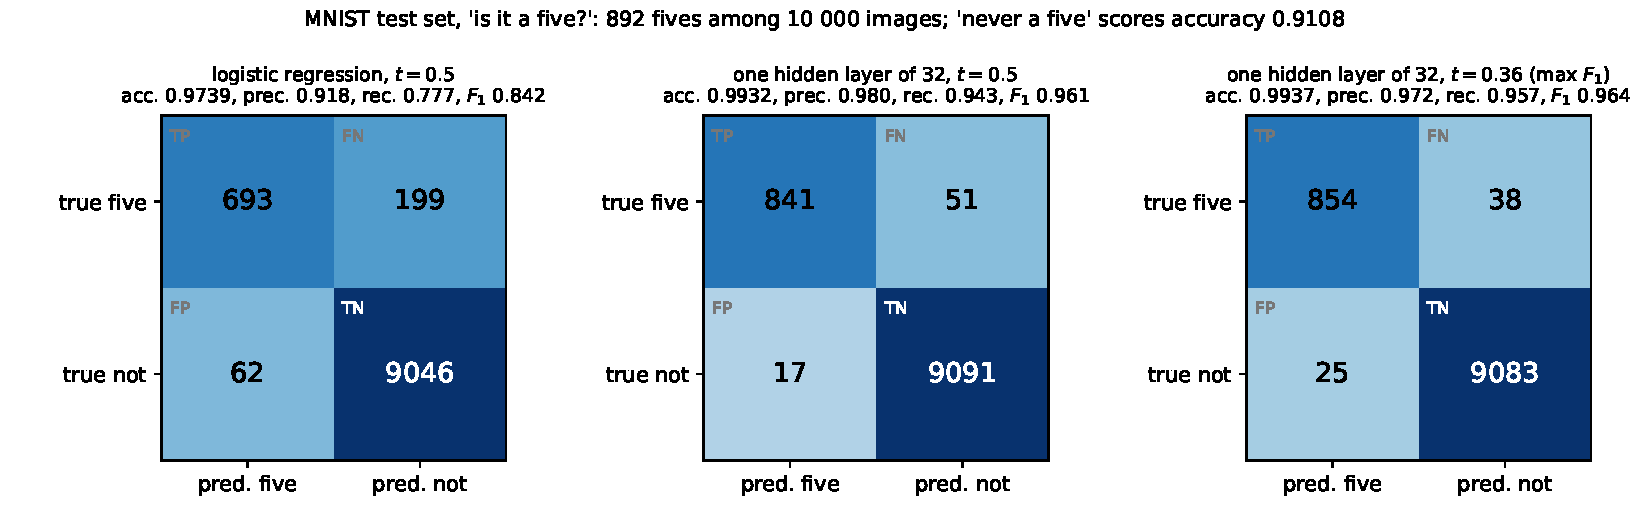
\includegraphics[width=0.9\textwidth]{week43_confusion}
\end{center}
\scriptsize
\begin{columns}[T]
\begin{column}{0.5\textwidth}
\textbf{Logistic regression}: $97.4\%$ accuracy sounds good; the matrix
says it \emph{misses $199$ of the $892$ fives} -- recall $0.78$ -- while
the $62$ false alarms keep the precision at $0.92$.  The one number hid the
asymmetry.  Against the free $91.1\%$ it has removed $71\%$ of the
remaining error.
\end{column}
\begin{column}{0.48\textwidth}
\textbf{One hidden layer}: $51$ missed, $17$ false alarms, recall $0.94$,
precision $0.98$, $F_1=0.961$, MCC $0.958$; $92\%$ of the error left by the
majority rule is gone.  Third panel: the same network with the threshold
moved to $0.36$ -- $13$ more fives found for $8$ more false alarms, the
best $F_1$.  Same model, different decision.
\end{column}
\end{columns}
\end{frame}

\begin{frame}[fragile]{The ROC curve and the AUC in code: one sorted pass}
\begin{columns}[T]
\begin{column}{0.43\textwidth}
\scriptsize
Every point of the curve from one sort: walking down the sorted scores,
every sample flagged adds one to TP (a positive) or to FP (a negative);
one point per distinct score, then the trapezoidal rule for the area.  Or
the rank formula of the previous frame, which needs no curve.  Both give
$0.97254$ and $0.99914$ for our two classifiers, and so does
\texttt{sklearn.metrics.roc\_auc\_score}; the curve equals
\texttt{roc\_curve(..., drop\_intermediate=False)} point for point.
\begin{block}{The precision--recall curve}
From the same sorted pass with $\mathrm{TP}/(\mathrm{TP}+\mathrm{FP})$ in
place of the false positive rate; its floor is the prevalence, $0.089$
here.
\end{block}
\end{column}
\begin{column}{0.55\textwidth}
\begin{lstlisting}
def roc_curve(y_true, scores):
    order = np.argsort(-scores, kind="mergesort")
    y, s = y_true[order], scores[order]
    tp, fp = np.cumsum(y == 1), np.cumsum(y == 0)
    last = np.r_[np.diff(s) != 0, True]  # per threshold
    tpr = np.r_[0.0, tp[last] / tp[-1]]
    fpr = np.r_[0.0, fp[last] / fp[-1]]
    return fpr, tpr, np.r_[np.inf, s[last]]

def roc_auc(y_true, scores):    # P(pos > neg)
    _, inv, cnt = np.unique(scores, return_inverse=True,
                            return_counts=True)
    first = np.cumsum(cnt) - cnt + 1
    ranks = (first + (cnt - 1) / 2)[inv]   # ties: mean rank
    n_pos = np.sum(y_true == 1)
    n_neg = len(y_true) - n_pos
    S = np.sum(ranks[y_true == 1])
    S -= n_pos * (n_pos + 1) / 2
    return S / (n_pos * n_neg)
\end{lstlisting}
\scriptsize
The precision--recall curve comes from the same sorted pass with
precision $=\mathrm{TP}/(\mathrm{TP}+\mathrm{FP})$ in place of the false
positive rate.  Unlike the ROC curve it \emph{does} depend on the
prevalence: its floor is the fraction of positives, $0.089$ here.
\end{column}
\end{columns}
\end{frame}

\begin{frame}{The four pictures (\texttt{week43\_metrics.pdf})}
\begin{center}
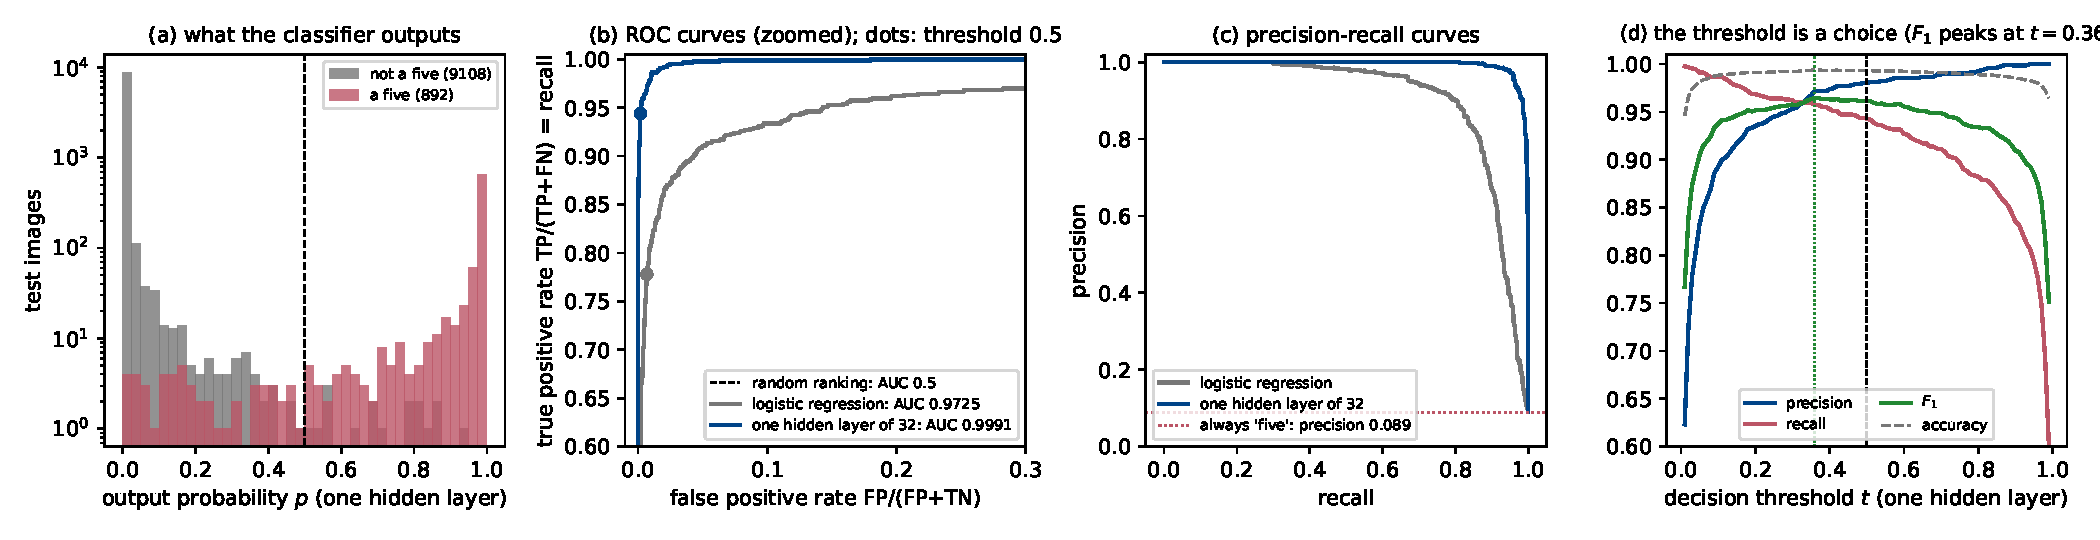
\includegraphics[width=0.99\textwidth]{week43_metrics}
\end{center}
\scriptsize
(a) The network's output on the test set, by class: most images sit at
$p\approx0$ or $p\approx1$, and the errors live in the thin middle -- a
threshold anywhere between $0.2$ and $0.6$ changes little.  (b) The ROC
curves, zoomed to the corner that matters: at a false positive rate of
$1\%$ the network has found $98\%$ of the fives, logistic regression $82\%$;
the dots are $t=0.5$.  (c) The precision--recall curves: logistic regression
cannot keep precision above $0.9$ beyond a recall of $0.8$; the network
holds $0.97$ to $0.96$.  (d) Precision, recall and $F_1$ against $t$ for the
network: accuracy (dashed) is flat and useless as a guide, $F_1$ peaks at
$t=0.36$, and the two curves cross -- there is no $t$ that is best for both.
\end{frame}

\begin{frame}{Choosing the threshold is choosing what an error costs}
\small
\begin{columns}[T]
\begin{column}{0.5\textwidth}
\begin{center}
\scriptsize
\begin{tabular}{@{}lccccc@{}}
\toprule
network at $t$ & TP & FN & FP & precision & recall\\
\midrule
$0.50$, convention & $841$ & $51$ & $17$ & $0.980$ & $0.943$\\
$0.36$, max $F_1$ & $854$ & $38$ & $25$ & $0.972$ & $0.957$\\
$0.11$, miss $=5$ alarms & $880$ & $12$ & $98$ & $0.900$ & $0.986$\\
\bottomrule
\end{tabular}
\end{center}
\scriptsize
Logistic regression under the same rule: $t=0.28$, recall $0.87$,
precision $0.81$ -- it cannot get both, which is what its AUC of $0.9725$
against $0.9991$ already said.
\end{column}
\begin{column}{0.48\textwidth}
\begin{block}{The procedure}
\scriptsize
\begin{enumerate}
  \item Decide, \emph{before} looking at the test set, what a false negative
        costs relative to a false positive.  That is a statement about the
        application and nobody else can make it for you.
  \item Choose $t$ on the \emph{validation} data (or by cross-validation,
        Section 2.12) to minimise that cost -- or to maximise $F_1$ when
        the two costs are equal and the classes are imbalanced.
  \item Report the confusion matrix at that $t$, plus the AUC, which does
        not depend on it.  Report the accuracy next to the majority-class
        accuracy or not at all.
\end{enumerate}
\end{block}
\begin{block}{What a threshold cannot do}
\scriptsize
Moving $t$ moves along the ROC curve; it cannot lift the curve.  The
$12$ fives the network still misses at $t=0.11$ have $p<0.11$: the model
ranks them below $98$ non-fives, and no decision rule fixes a ranking.
Fixing the ranking means a better model, more data, or training with class
weights (the notebox of Section 5.12).
\end{block}
\end{column}
\end{columns}
\end{frame}

\begin{insight}[the threshold moved from $0.5$ to $0.11$ -- did the classifier change?]
\question{The third row of the table has a very different confusion matrix
from the first: $29$ more fives found, $81$ more false alarms.  Which of the
following changed, and which did not: the weights, the output
probabilities, the ranking of the test images, the ROC curve, the AUC, the
precision--recall curve, the accuracy?}
\answer{Nothing about the model changed: weights, probabilities, ranking,
ROC curve, AUC and precision--recall curve are identical, because all of
them are properties of the scores and the threshold enters none of them.
Only the \emph{operating point} on those curves moved, and with it every
number computed from the four counts: accuracy ($0.9932\to0.9890$ -- it
went \emph{down} while the recall went up, which is why accuracy is a poor
guide under imbalance), precision, recall, $F_1$.  This is the division to
keep in mind for Project 2: the AUC and the curves evaluate the
\emph{model}; the confusion matrix evaluates the model \emph{together with
a decision rule}, and a report should say which rule.}
\end{insight}

\begin{frame}{Ten classes: the confusion matrix of the softmax network (\texttt{week43\_confusion10.pdf})}
\begin{center}
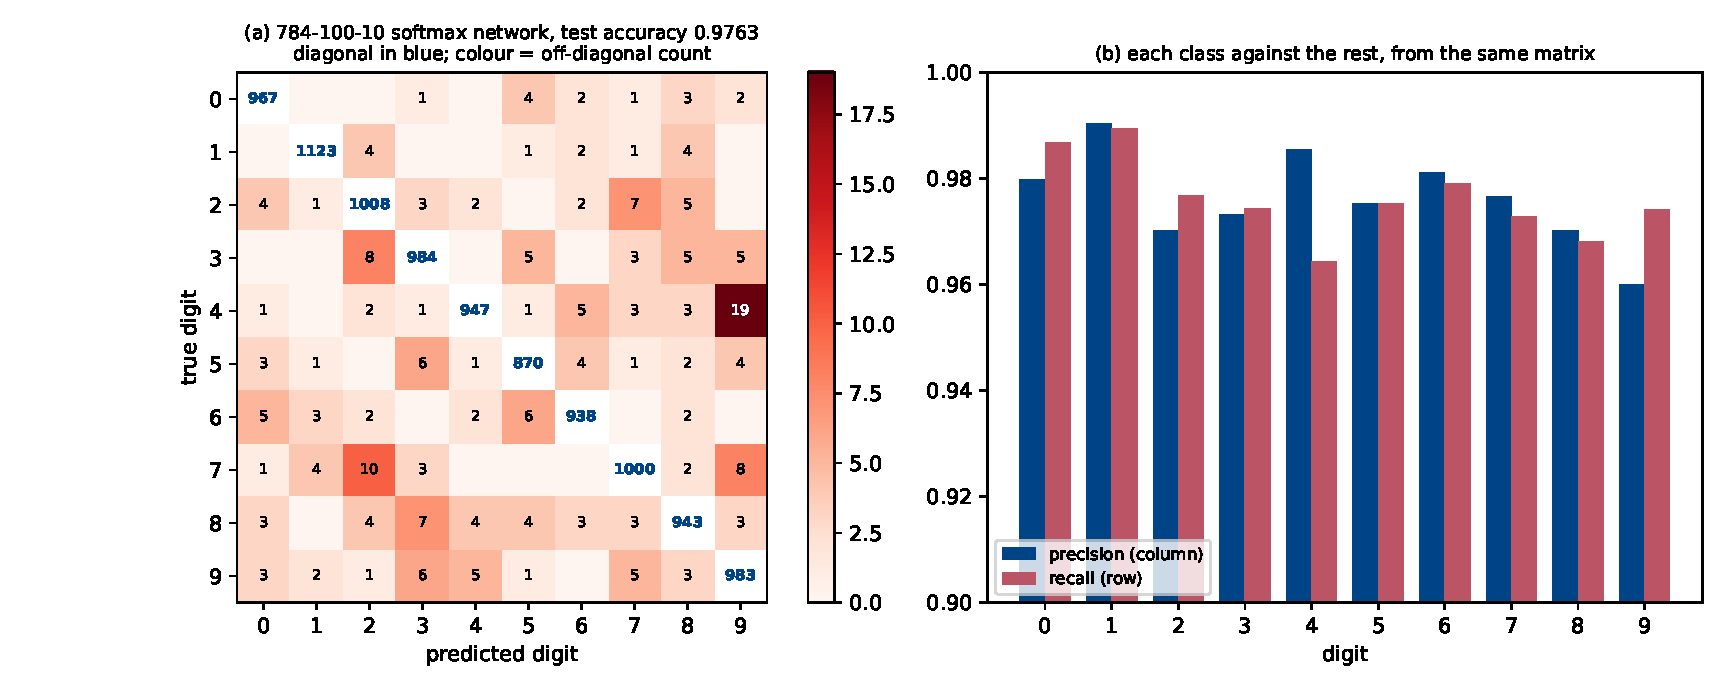
\includegraphics[width=0.82\textwidth]{week43_confusion10}
\end{center}
\scriptsize
\begin{columns}[T]
\begin{column}{0.5\textwidth}
The $784\to100\to10$ ReLU network of weeks 41--42, twenty epochs, test
accuracy $0.9763$ -- the same number as last week, to the digit.  The matrix
says \emph{where} the $237$ errors are: $19$ fours read as nines, $10$ sevens
as twos, $8$ sevens as nines, $8$ threes as twos, $7$ eights as threes.
Nines are the hardest to be sure of (precision $0.960$), fours the easiest
to miss (recall $0.964$).
\end{column}
\begin{column}{0.48\textwidth}
Each class against the rest is a $2\times2$ matrix read off the big one:
the row gives the recall of a class, the column its precision.  The
``everything else'' column is why a $97.6\%$ accuracy is compatible with a
$96\%$ precision on the nines.  Project 2 asks for this matrix and for its
interpretation; the $4\to9$ and $7\to9$ confusions are what the second hour
is about.
\end{column}
\end{columns}
\end{frame}

\begin{frame}{Other ways of presenting classification results, and an error bar}
\small
\begin{columns}[T]
\begin{column}{0.5\textwidth}
\begin{block}{Beyond the matrix, the ROC and the PR curve}
\scriptsize
\begin{itemize}
  \item \textbf{The probability histograms} by class, panel (a): the first
        thing to look at.  A good classifier separates them; the overlap is
        the error, whatever $t$.
  \item \textbf{Calibration (reliability) diagrams}: bin the test images by
        $p$ and plot the fraction of fives in each bin against $p$.  A
        calibrated classifier lies on the diagonal; then $p$ means what it
        says, and the threshold can be set from costs alone.
  \item \textbf{Proper scoring rules} that use $p$ and not a decision: the
        test cross entropy (log loss) and the Brier score
        $\frac{1}{n}\sum_i(p_i-y_i)^{2}$.
  \item \textbf{Average precision}, the area under the PR curve, when the
        positives are rare and the ROC curve looks flattering.
  \item \textbf{Per-class precision and recall} from the rows and columns
        of the $K\times K$ matrix (\texttt{classification\_report}), and
        the macro average when the classes are imbalanced.
\end{itemize}
\end{block}
\end{column}
\begin{column}{0.48\textwidth}
\begin{block}{Every one of these numbers has an error bar}
\scriptsize
An accuracy $\hat{p}$ on $n$ test images is a binomial proportion with
standard error $\sqrt{\hat{p}(1-\hat{p})/n}$ (Eq.~2.24): for
$0.9763$ on $10\,000$ images, $\pm0.0015$; for $0.958$ on the $143$
Wisconsin test samples of Section 5.13, $\pm0.017$.  Two models that differ
by less than that are not distinguishable by that test set.  The recall of
the fives rests on $892$ images: $\pm0.008$.  Cross-validation
(Section 2.12) gives the honest spread: in Section 5.13 the cross-validated
accuracy was $0.981\pm0.025$ against $0.958$ on the test set, a difference
within one and a half standard errors.
\end{block}
\begin{block}{In Project 2}
\scriptsize
Confusion matrix on the full $10\,000$ test images, used once; the
hyperparameters chosen on validation data; the accuracy next to its
standard error and next to the $10\%$ guess and the $\approx92\%$ of
logistic regression; and when you compare two networks, say whether the
difference exceeds the error bar.
\end{block}
\end{column}
\end{columns}
\end{frame}

\begin{insight}[an accuracy of $97.4\%$ -- good or bad?]
\question{Logistic regression reached a test accuracy of $0.9739$ on ``is
it a five?''.  Is that a good classifier?  What three numbers would you
want next to it before answering, and what do they say here?}
\answer{On its own the number says little.  Next to it: (1) the majority
accuracy, $0.9108$ -- so the model removed $71\%$ of the error that was
left, which is real but far from the $92\%$ of the one-hidden-layer
network; (2) the recall, $0.78$ -- it misses more than one five in five,
which the accuracy hides because fives are $9\%$ of the images; (3) the
AUC, $0.9725$ against $0.9991$ -- the \emph{ranking} is worse, so no
threshold will rescue it: at the recall of the network ($0.94$) its
precision has fallen below $0.8$.  The honest sentence is ``logistic
regression finds $78\%$ of the fives with $8\%$ false alarms; the network
finds $94\%$ with $2\%$'' -- and the honest figure is the pair of
confusion matrices, which is why Project 2 asks for them.}
\end{insight}

%% ====================================================================
%% Part 3: convolutional neural networks (45 min)
%% ====================================================================

\begin{frame}{Why not simply use a dense layer?  (Section 10.1)}
\small
\begin{columns}[T]
\begin{column}{0.5\textwidth}
\begin{block}{What the flattening threw away}
\scriptsize
The network of Chapter 8 turns a $28\times28$ image into a vector of $784$
numbers and multiplies it by a dense matrix.  Permute the pixels of
\emph{every} image by one fixed permutation and the network learns exactly
as well: nothing in an affine map knows that pixel $(i,j)$ sits next to
pixel $(i,j+1)$.  Images, sound and spectra have an \emph{ordering} along
one or more axes and a \emph{channel} axis (red, green, blue), and a vector
records neither.
\end{block}
\begin{block}{The objection is one of counting, (10.1)--(10.2)}
\scriptsize
A colour image of side $L$ into a hidden layer of the same size:
$N_{\mathrm{dense}}=(3L^{2})^{2}=9L^{4}$ -- $9.4$ million for the $32\times32$
images of CIFAR-10, $1.4\times10^{10}$ for a $200\times200$ photograph.  A
convolutional layer with $K$ filters of extent $F$ on $C$ channels has
\[
  N_{\mathrm{conv}}=K\,(CF^{2}+1)\qquad(10.2)
\]
weights, \emph{independent of the image size}: $1792$ for $F=3$, $C=3$,
$K=64$ whether the image is $32\times32$ or $4096\times4096$.
\end{block}
\end{column}
\begin{column}{0.48\textwidth}
\begin{center}
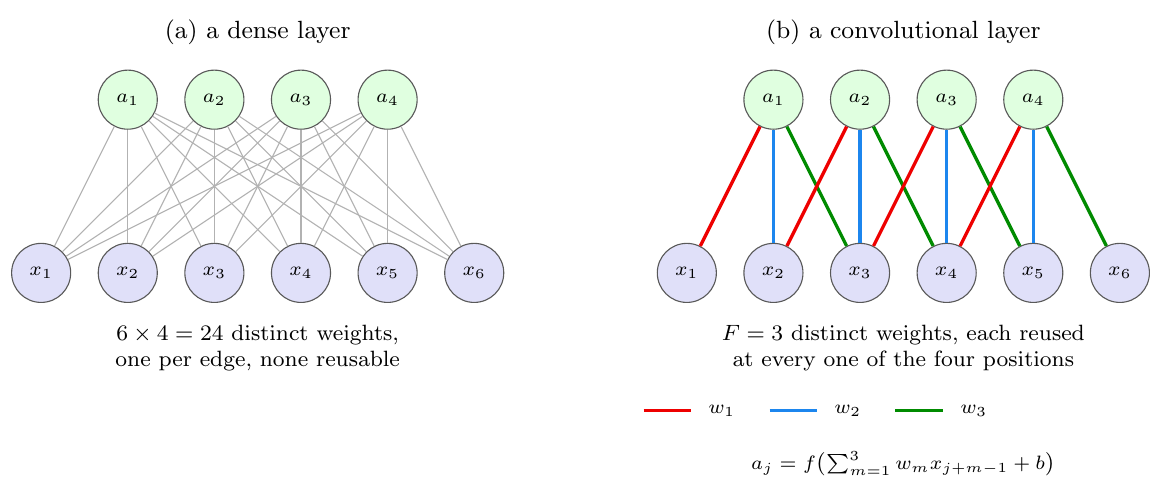
\includegraphics[width=0.98\textwidth]{10-connect}\\
\scriptsize Book Figure 10.1.
\end{center}
\begin{block}{The two assumptions that buy the saving}
\scriptsize
\textbf{Locality}: an output depends on a small neighbourhood of the input
-- the three coloured edges into each $a_j$.  \textbf{Parameter sharing}:
the same weights $w_1,w_2,w_3$ at every position -- the three colours
repeat.  Twenty-four weights become three, and the three do not grow when
the input is lengthened.  Both are properties of the \emph{data}, not of
the method: for a table of unrelated clinical measurements neither holds
and a convolutional layer is an actively bad choice.
\end{block}
\end{column}
\end{columns}
\end{frame}

\begin{frame}[fragile]{Convolution is polynomial multiplication (Sections 10.2--10.2.1)}
\begin{columns}[T]
\begin{column}{0.5\textwidth}
\scriptsize
For sequences, Eq.~(10.4): $y(i)=(x*w)(i)=\sum_{k}w(k)\,x(i-k)$,
commutative (substitute $k\to i-k$) and linear in each argument.  The
quickest intuition has nothing to do with images.  Multiply
$p(t)=\alpha_0+\alpha_1t+\alpha_2t^{2}$ by
$s(t)=\beta_0+\beta_1t+\beta_2t^{2}+\beta_3t^{3}$ and collect terms
(10.6):
\begin{align*}
  \delta_0&=\alpha_0\beta_0,\quad
  \delta_1=\alpha_1\beta_0+\alpha_0\beta_1,\quad
  \delta_2=\alpha_0\beta_2+\alpha_1\beta_1+\alpha_2\beta_0,\\
  \delta_3&=\alpha_1\beta_2+\alpha_2\beta_1+\alpha_0\beta_3,\quad
  \delta_4=\alpha_2\beta_2+\alpha_1\beta_3,\quad
  \delta_5=\alpha_2\beta_3 .
\end{align*}
Every line has the same shape: the indices of the two factors sum to the
index of the result,
\[
  \delta_l=\sum_k\alpha_k\beta_{l-k}=(\alpha*\beta)_l\qquad(10.7).
\]
\emph{Polynomial multiplication is discrete convolution}: not an analogy,
the coefficient sequences convolve.
\end{column}
\begin{column}{0.48\textwidth}
\begin{lstlisting}
alpha = np.array([1.0, 2.0, 3.0])        # p(t)
beta = np.array([4.0, -1.0, 0.5, 2.0])   # s(t)
np.polynomial.polynomial.polymul(alpha, beta)   # [4. 7. 10.5 0. 5.5 6.]
np.convolve(alpha, beta)                        # the same
toeplitz_matrix(alpha, 4) @ beta                # the same
\end{lstlisting}
\begin{block}{The Toeplitz matrix of the third line, Eq.~(10.8)}
\scriptsize
Linearity in $\bm{\beta}$ means a matrix, $(\bm{T}_w)_{ij}=w_{i-j}$:
\[
  \setlength{\arraycolsep}{2pt}
  \bm{T}_{\alpha}=
  {\tiny\begin{bmatrix}
    1&0&0&0\\ 2&1&0&0\\ 3&2&1&0\\ 0&3&2&1\\ 0&0&3&2\\ 0&0&0&3
  \end{bmatrix}},\qquad
  \bm{T}_{\alpha}\bm{\beta}=\bm{\alpha}*\bm{\beta}.
\]
Constant descending diagonals: a \emph{Toeplitz} matrix (Definition
10.1).  Theorem 10.2: a matrix is a convolution \emph{if and only if} it is
Toeplitz.  Locality makes it banded, sharing makes each diagonal constant
-- so the two assumptions are not merely convenient, they are
\emph{exhaustive}.
\end{block}
\end{column}
\end{columns}
\end{frame}

\begin{frame}{Two remarks the theorem brings with it (Sections 10.2.2--10.2.3)}
\small
\begin{columns}[T]
\begin{column}{0.5\textwidth}
\begin{center}
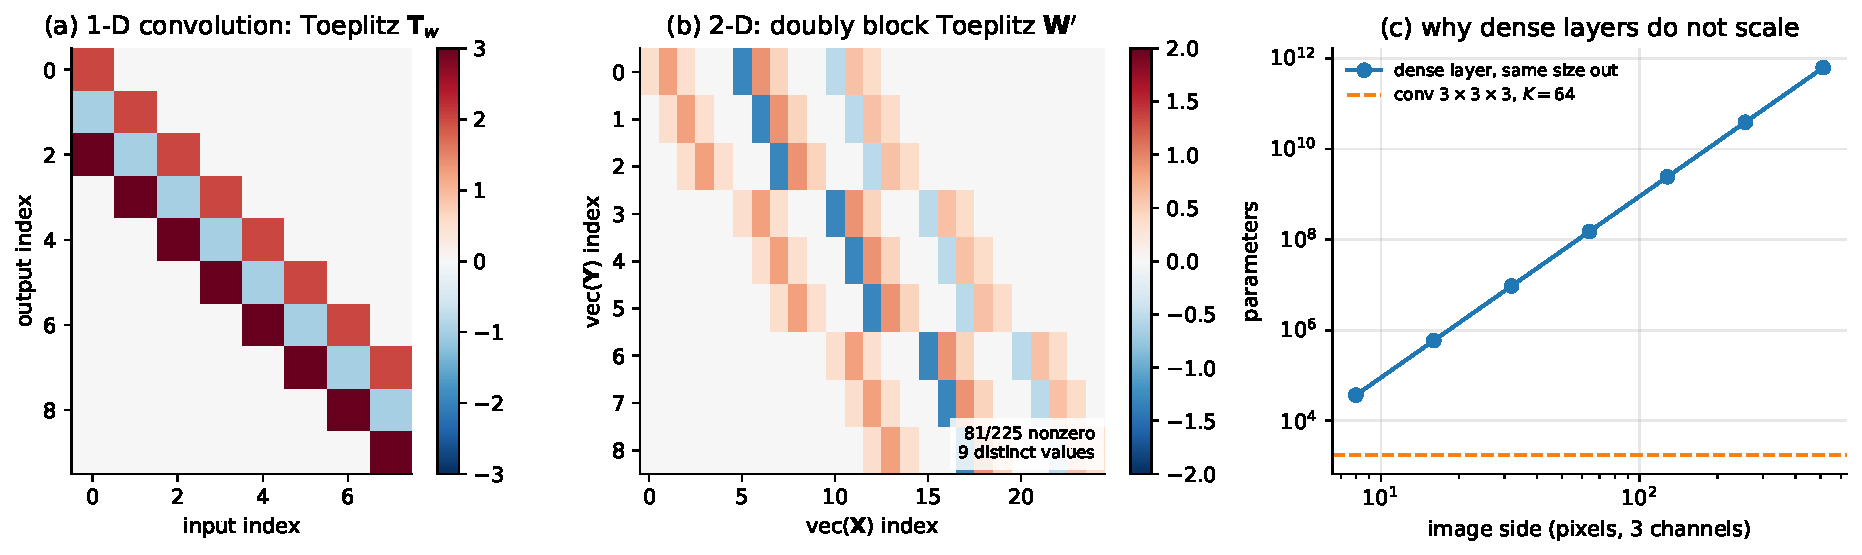
\includegraphics[width=0.98\textwidth]{convolution_structure}\\
\scriptsize Book Figure 10.3: (a) a one-dimensional kernel of length three
as a Toeplitz matrix; (b) the doubly block Toeplitz matrix of a $3\times3$
kernel on a $5\times5$ image, nine numbers in $81$ of $225$ positions;
(c) parameters per layer against image side.
\end{center}
\end{column}
\begin{column}{0.48\textwidth}
\begin{block}{Do not build these matrices}
\scriptsize
The Toeplitz form is for reasoning.  Storing $\bm{T}_w$ costs
$\mathcal{O}(n^{2})$; evaluating (10.4) directly costs $\mathcal{O}(nm)$
with $m\ll n$; and by the fast Fourier transform $\mathcal{O}(n\log n)$.
The code of Section 10.7 never forms one -- exactly as Thomas' algorithm
never formed the dense matrix an hour ago.
\end{block}
\begin{block}{The convolution theorem (Theorem 10.3)}
\scriptsize
In the periodic case the Toeplitz matrix is \emph{circulant}, and every
circulant matrix has the same eigenvectors, the Fourier modes
$\omega^{kj}$:
\[
  \bm{C}=\bm{F}^{*}\operatorname{diag}(\hat{\bm{c}})\bm{F},\qquad
  \widehat{\bm{c}*\bm{x}}=\hat{\bm{c}}\odot\hat{\bm{x}}\quad(10.10,\ 10.11).
\]
Convolution is multiplication in Fourier space: a convolutional layer
multiplies each frequency by one learned number -- it is a learned filter
bank.  Why not build the network there?  Because kernels are tiny ($9n$
operations for $F=3$ beats two transforms until $F\approx11$), and because
the non-linearity between layers is elementwise \emph{in space}: the
architecture alternates a map diagonal in frequency with a map diagonal in
space, and that is where its power comes from.
\end{block}
\end{column}
\end{columns}
\end{frame}

\begin{frame}{Padding, and what libraries actually compute (Sections 10.2.4--10.2.5)}
\small
\begin{columns}[T]
\begin{column}{0.5\textwidth}
\begin{block}{Indices out of range, (10.12)}
\scriptsize
With a filter of length $m$ on an input of length $n$,
$y(i)=\sum_{k=0}^{m-1}w(k)x(i-k)$ asks for $x(-1)$ at $i=0$.  Pad with $P$
zeros at each end:
\begin{center}
\begin{tabular}{@{}lll@{}}
\toprule
name & $P$ & output length\\
\midrule
valid & $0$ & $n-m+1$\\
same & $(m-1)/2$ & $n$\\
full & $m-1$ & $n+m-1$\\
\bottomrule
\end{tabular}
\end{center}
Zeros are a choice and they are visible: outputs near the border are
computed from fewer genuine inputs than outputs in the middle.
\end{block}
\end{column}
\begin{column}{0.48\textwidth}
\begin{block}{Cross-correlation, (10.13)}
\scriptsize
Equation (10.4) reads the input \emph{backwards}, $x(i-k)$, which means
flipping the kernel before sliding it.  When the kernel is learned that is
pointless, so every library computes
\[
  y(i)=\sum_k w(k)\,x(i+k)
\]
and calls it convolution.  We follow the convention from here on.  It
changes nothing about what the layer can represent -- the network learns
the reflected filter -- and it matters only when the kernel is prescribed
(a Gaussian blur, a derivative filter) or compared with a textbook formula.
Cross-correlation is \emph{not} commutative: the symmetry between filter
and input of the polynomial example is lost.
\end{block}
\begin{block}{A sanity check we do in a moment}
\scriptsize
Our own four-line \texttt{cross\_correlate2d} agrees with
\texttt{scipy.signal.correlate2d(..., mode="valid")} to $4\times10^{-16}$.
\end{block}
\end{column}
\end{columns}
\end{frame}

\begin{frame}{Two dimensions, channels and the convolutional layer (Section 10.3)}
\scriptsize
Input $\bm{X}\in\mathbb{R}^{C\times H\times W}$ with $C$ channels; $K$
filters, \emph{each} of shape $C\times F\times F$, in
$\bm{W}\in\mathbb{R}^{K\times C\times F\times F}$ with biases
$b\in\mathbb{R}^{K}$.  For $k=0,\dots,K-1$, with stride $S$ and padding
$P$, then $A=f(Z)$ elementwise:
\[
  \boxed{\;Z(k,i,j)=\sum_{c=0}^{C-1}\sum_{m=0}^{F-1}\sum_{n=0}^{F-1}
    X\bigl(c,\,Si+m-P,\;Sj+n-P\bigr)\,W(k,c,m,n)+b(k)\;}\qquad(10.16)
\]
\begin{columns}[T]
\begin{column}{0.5\textwidth}
\scriptsize
\begin{block}{Three things to read off (10.16)}
\begin{enumerate}
  \item The sum over $c$ runs over \emph{all} input channels: a filter is a
        block spanning the whole depth, not an $F\times F$ patch, which is
        why nothing on the left carries a $c$.
  \item $i,j$ range over output positions, $m,n$ over the filter: the filter
        is small, the output is large.
  \item $W$ does not depend on $i$ or $j$: that is parameter sharing,
        written out.
\end{enumerate}
\end{block}
This is the layer $\bm{Z}^{l}=\bm{A}^{l-1}\bm{W}^{l}+\bm{b}^{l}$ of week 41
with a very sparse, very repetitive $\bm{W}$ -- and the backward pass of
Section 10.6 is the four equations of week 41 applied to it.
\end{column}
\begin{column}{0.48\textwidth}
\begin{center}
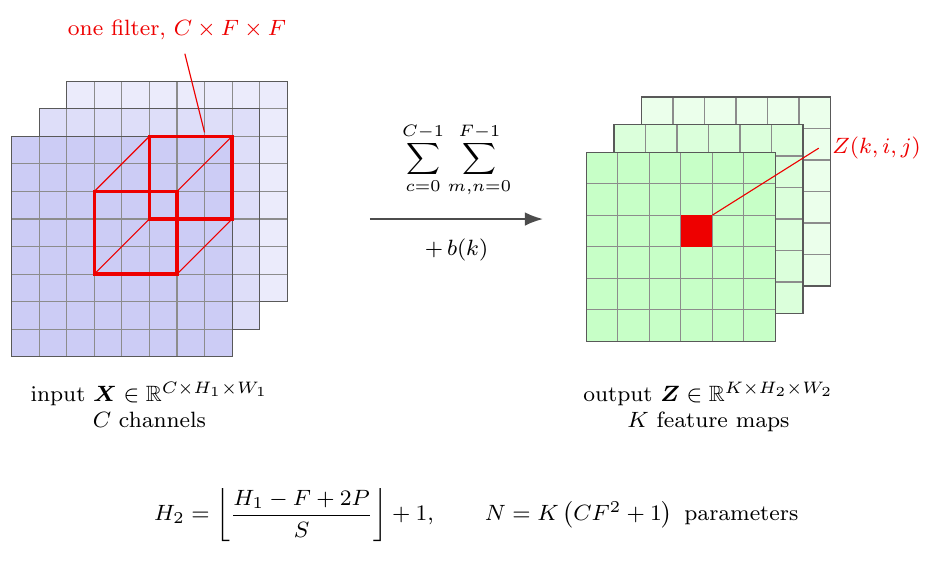
\includegraphics[width=0.98\textwidth]{10-convlayer}\\
\scriptsize Book Figure 10.2: one filter spans the depth, produces one value
$Z(k,i,j)$; sliding it fills one feature map; $K$ filters give $K$ maps.
\end{center}
\end{column}
\end{columns}
\end{frame}

\begin{frame}{Output size and parameter count: Proposition 10.4}
\small
\begin{columns}[T]
\begin{column}{0.5\textwidth}
\begin{block}{Convolution arithmetic, (10.17)--(10.18)}
\scriptsize
Input $H_1\times W_1\times C$, $K$ filters of extent $F$, stride $S$,
padding $P$: the output has depth $K$ and
\[
  H_2=\Bigl\lfloor\frac{H_1-F+2P}{S}\Bigr\rfloor+1,\qquad
  W_2=\Bigl\lfloor\frac{W_1-F+2P}{S}\Bigr\rfloor+1,
\]
with $N=K(CF^{2}+1)$ trainable parameters.  \emph{Proof}: the padded input
has $H_1+2P$ rows; the filter's first row $t$ must satisfy
$t+F-1\le H_1+2P-1$, and the admissible multiples of $S$ in
$[0,H_1+2P-F]$ number $\lfloor(H_1+2P-F)/S\rfloor+1$.  The floor is not
decoration: when $S$ does not divide, the last rows are silently
discarded, which is why $F=3,S=1,P=1$ and $F=5,S=1,P=2$ (both
$H_2=H_1$) are the usual choices.
\end{block}
\begin{block}{Example 10.5, and our own}
\scriptsize
$32\times32\times3$, $K=10$, $F=5$, $S=1$, $P=0$: $H_2=W_2=28$, output
$28\times28\times10$, $10\times(75+1)=760$ parameters.  A dense layer with
the same $7840$ outputs: $3072\times7840\approx2.4\times10^{7}$.\\[2pt]
MNIST $28\times28\times1$, $K=8$, $F=3$, $S=1$, $P=1$: output
$28\times28\times8$ and \textbf{80 parameters}; the dense $784\to100$ layer
of week 41 has $78\,500$.
\end{block}
\end{column}
\begin{column}{0.48\textwidth}
\begin{block}{The unrolled matrix, (10.19)}
\scriptsize
Equation (10.16) is linear in $\bm{X}$, so it is a matrix.  A $3\times3$
input flattened to $\bm{X}'\in\mathbb{R}^{9}$ and a $2\times2$ filter:
\[
  \setlength{\arraycolsep}{1.5pt}
  \bm{W}'=
  {\tiny
  \begin{bmatrix}
    w_{00}&w_{01}&0&w_{10}&w_{11}&0&0&0&0\\
    0&w_{00}&w_{01}&0&w_{10}&w_{11}&0&0&0\\
    0&0&0&w_{00}&w_{01}&0&w_{10}&w_{11}&0\\
    0&0&0&0&w_{00}&w_{01}&0&w_{10}&w_{11}
  \end{bmatrix}}
\]
-- doubly block Toeplitz, four numbers in thirty-six positions.  This is
what the $784\times100$ matrix of week 41 would have to look like to be a
convolution: almost all zeros, and the non-zeros repeated.  A dense layer
\emph{could} learn it, from enough data; the convolutional layer
\emph{is} it, from the start.
\end{block}
\begin{block}{Where the parameters went}
\scriptsize
Into the \emph{depth} -- many layers, many filters each -- and into the
dense layer at the end, which dominates the count (Section 10.10.4).
\end{block}
\end{column}
\end{columns}
\end{frame}

\begin{frame}[fragile]{Our demonstration: a five and three filters (\texttt{week43\_convolution})}
\begin{center}
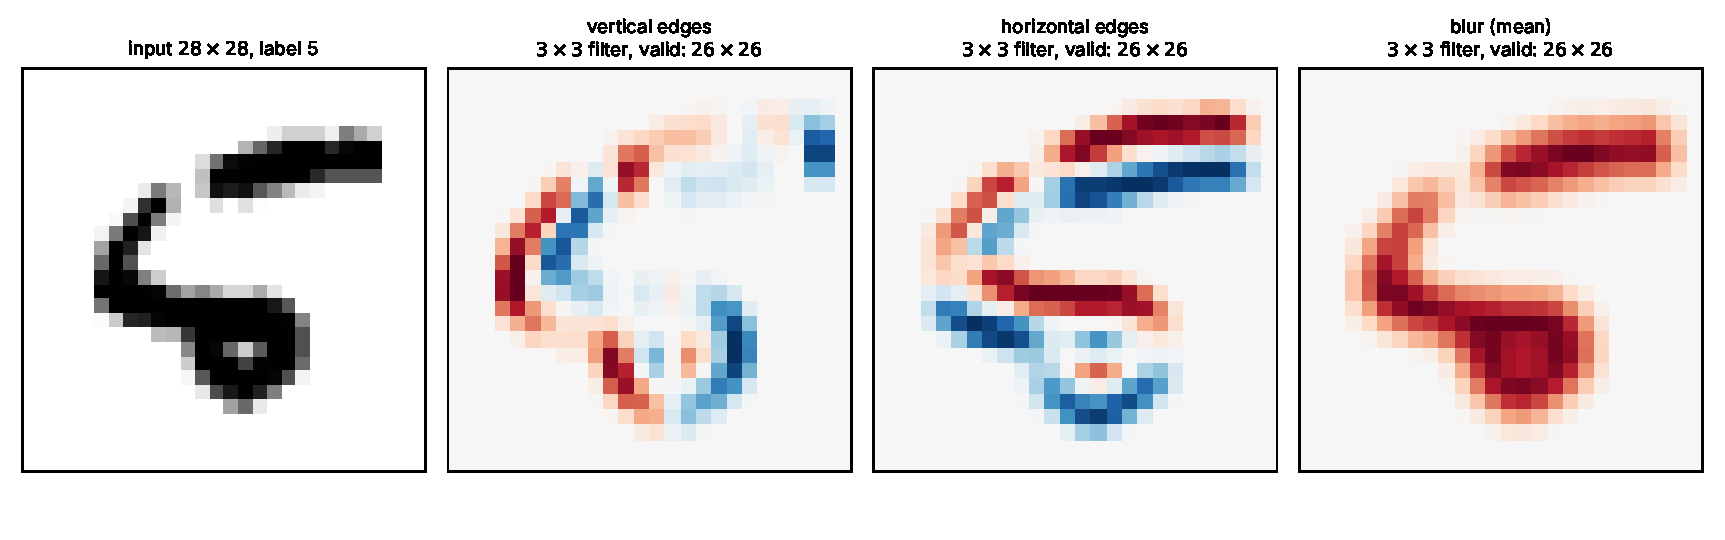
\includegraphics[width=0.78\textwidth]{week43_convolution}
\end{center}
\begin{columns}[T]
\begin{column}{0.56\textwidth}
\begin{lstlisting}
def cross_correlate2d(X, W, stride=1, padding=0): # (10.16)
    if padding: X = np.pad(X, padding)
    F = W.shape[0]
    H2 = (X.shape[0] - F) // stride + 1
    W2 = (X.shape[1] - F) // stride + 1
    Y = np.zeros((H2, W2))
    for i in range(H2):
        for j in range(W2):
            r, c = stride * i, stride * j
            Y[i, j] = np.sum(X[r:r + F, c:c + F] * W)
    return Y
\end{lstlisting}
\end{column}
\begin{column}{0.42\textwidth}
\scriptsize
Three \emph{prescribed} $3\times3$ filters -- the Sobel derivative
$\begin{bmatrix}-1&0&1\\-2&0&2\\-1&0&1\end{bmatrix}$, its transpose, and
the $\tfrac{1}{9}$ mean -- on test image 8 (a five), by the loop on the
left (agrees with \texttt{scipy.signal.correlate2d} to $4\times10^{-16}$).
Valid padding: $28\to26$.  The vertical-edge map is positive (red) where
the ink starts along a row and negative (blue) where it ends; the
horizontal one the same for the strokes; the blur is a low-pass filter.
Each map is one \emph{feature map}, Eq.~(10.16) with $C=K=1$; a layer with
$K=3$ filters makes all three at once, $30$ parameters.  A trained network
learns such filters from the data (Figure 10.8c).
\end{column}
\end{columns}
\end{frame}

\begin{insight}[why is the map $26\times26$, and what does the vertical-edge filter compute?]
\question{The input is $28\times28$ and the feature maps are $26\times26$.
Why, and what would $P=1$ or $S=2$ give?  Why does the first filter light
up on the \emph{vertical} strokes of the five although its rows read
$(-1,0,1)$?  And what does the activation function $f$ of Eq.~(10.16) do
to such a map?}
\answer{Proposition 10.4 with $F=3$, $S=1$, $P=0$: $H_2=28-3+1=26$.  With
$P=1$ (``same'') the map stays $28\times28$; with $S=2$ it is
$\lfloor25/2\rfloor+1=13$ -- every second row and column, computed with
the same nine weights.  The filter is a central difference in the
horizontal direction, $\partial X/\partial x$, smoothed vertically by the
$(1,2,1)$ weights: it is large where the intensity \emph{changes along a
row}, which is at a vertical stroke -- the left and right edges of the
ink -- and zero on a horizontal stroke, where every row is constant.  The
sign gives the direction of the change (ink begins, ink ends); a ReLU
after the layer keeps only one direction, so one filter and its negative
would be needed to keep both -- which is exactly the opposed-sign pairs a
trained first layer ends up with (Figure 10.8c).}
\end{insight}

\begin{frame}{Where this is going: tomorrow, the exercises, Project 2, next week}
\small
\begin{columns}[T]
\begin{column}{0.5\textwidth}
\begin{block}{Tomorrow: the measures once more, then one case}
\footnotesize
First the worked screening example of today in full detail, measure by
measure, in plenum; then \emph{one} case in \texttt{week43tuesday.ipynb}:
your own confusion matrix, ROC curve and AUC, written from the definitions
and checked against \texttt{scikit-learn}, on ``is it an eight?'' with the
small digits set (seconds per run) and logistic regression against a
one-hidden-layer network from your own code -- the structure of this
week's exercises.
\end{block}
\begin{block}{Exercises week 43 (deadline Friday October 23)}
\footnotesize
Exercise 1: the metric functions, checked against the library.  Exercise
2: MNIST, one digit against the rest, with your Project 2 classifiers --
confusion matrix, ROC and AUC.  Exercise 3 (optional): the $10\times10$
matrix.  No validation sets or cross-validation yet: how to cross-validate
your Project 2 network is the topic of next week's Tuesday session and
exercises.  Declare your use of LLMs.
\end{block}
\end{column}
\begin{column}{0.48\textwidth}
\begin{block}{Project 2 (deadline November 6)}
\footnotesize
Part e) asks for logistic regression as the baseline and for the confusion
matrix on the full MNIST test set, with its interpretation -- Part 2 of
today.  Part 1 (the differential equations) is not part of the project.
\end{block}
\begin{block}{Next Monday, week 44: Chapter 10 continued}
\footnotesize
Equivariance -- convolution is the \emph{only} linear map that commutes
with translation (10.4); pooling and the receptive field (10.5); the
backward pass through a convolution and a pool (10.6); the implementation
with \texttt{im2col} (10.7) and the experiment of Section 10.8.
\end{block}
\begin{block}{Reading}
\footnotesize
Sections 9.5, 9.10 and 1.14; Sections 5.12--5.13; Chapter 10, Sections
10.1--10.3.  Then 10.4--10.5 for next week.
\end{block}
\end{column}
\end{columns}
\end{frame}

\begin{frame}{Summary of week 43}
\small
\begin{columns}[T]
\begin{column}{0.5\textwidth}
\begin{block}{One equation, three ways}
\footnotesize
\begin{itemize}
  \item Hard: conditions in the ansatz, exact and free.  Soft: in the
        cost, a $\lambda$ to choose, four times worse at best, the only
        option when no ansatz exists.  Thomas: tridiagonal LU, $8n$ flops,
        $2\times10^{-9}$ in $11$ ms -- the network is not for problems that
        have one (9.9).
\end{itemize}
\end{block}
\begin{block}{Reading a classifier}
\footnotesize
\begin{itemize}
  \item Four counts, two kinds of error.  Accuracy is
        $\pi\,\mathrm{recall}+(1-\pi)\,\mathrm{specificity}$ -- blind to the
        rare class; recall asks about the misses, precision about the false
        alarms, $F_1$ is small if either is; MCC is their correlation.
  \item ROC and AUC judge the ranking, blind to threshold and prevalence;
        the PR curve is not.  Choose $t$ from costs on validation data;
        report the matrix at that $t$, the AUC, and an error bar
        $\sqrt{\hat p(1-\hat p)/n}$.  Train on the cross entropy, report the
        rest.
\end{itemize}
\end{block}
\end{column}
\begin{column}{0.48\textwidth}
\begin{block}{Convolutional networks, the first hour}
\footnotesize
\begin{itemize}
  \item A dense layer on an image costs $9L^{4}$ parameters and knows
        nothing about neighbours; locality and sharing give $K(CF^{2}+1)$,
        independent of the image size.
  \item Convolution is polynomial multiplication, a Toeplitz matrix, and
        diagonal in Fourier space; libraries compute cross-correlation.
        The layer (10.16): filters span the depth; sizes (10.17), parameters
        (10.18).
  \item Three prescribed filters on a five: a feature map is a derivative
        or an average of the image; a trained layer learns the filters.
        Next week: why convolution is the \emph{only} translation-equivariant
        linear map, pooling, and the experiment that shows what the
        architecture buys.
\end{itemize}
\end{block}
\end{column}
\end{columns}
\end{frame}

\end{document}
